% tutorial.tex — End-to-End QCG tutorial (mirrors notebook 04)
% Technical customer presentation. Uses the canonical QCi beamer template.
%
% Compile: pdflatex tutorial.tex (twice for frame numbers)
\documentclass[aspectratio=169,11pt]{beamer}

% =============================================================
% Theme + brand colors
% =============================================================
\usetheme{Madrid}
\setbeamertemplate{navigation symbols}{}

\usepackage[table]{xcolor}
\definecolor{QCIcol1}{HTML}{211D53}
\definecolor{QCIcol2}{HTML}{908FA8}
\definecolor{QCIcol3}{HTML}{D3DAE6}
\definecolor{QCIcol4}{HTML}{E8ECF2}
\definecolor{QCIcol5}{HTML}{F6F7FA}
\definecolor{qciorange}{RGB}{220,120,20}
\definecolor{qcigreen}{RGB}{40,140,60}
\definecolor{qciblue}{RGB}{0,70,130}
\definecolor{qciteal}{RGB}{0,128,128}

\setbeamercolor{palette primary}   {bg=QCIcol1,           fg=white}
\setbeamercolor{palette secondary} {bg=QCIcol2,           fg=white}
\setbeamercolor{palette tertiary}  {bg=QCIcol1!70,        fg=white}
\setbeamercolor{palette quaternary}{bg=QCIcol1,           fg=white}
\setbeamercolor{structure}         {fg=QCIcol1}
\setbeamercolor{block title}       {bg=QCIcol3,           fg=QCIcol1}
\setbeamercolor{block body}        {bg=QCIcol5}
\setbeamercolor{block title alerted}{bg=qciorange!20,     fg=qciorange!70!black}
\setbeamercolor{block body alerted} {bg=qciorange!5}
\setbeamercolor{block title example}{bg=qcigreen!15,      fg=qcigreen!70!black}
\setbeamercolor{block body example} {bg=qcigreen!5}
\setbeamercolor{alerted text}      {fg=qciorange}
\setbeamercolor{example text}      {fg=qcigreen!70!black}
\setbeamercolor{section in toc}    {fg=QCIcol1}
\setbeamercolor{subsection in toc} {fg=QCIcol2}
\setbeamercolor{frametitle}        {fg=white}

\usepackage{anyfontsize}
\usepackage[oldstyle,default]{raleway}
\usefonttheme{default}

\usepackage{amsmath,amssymb}
\usepackage{booktabs}
\usepackage{array}
\usepackage{graphicx}
\usepackage{tikz}
\usetikzlibrary{calc,positioning,arrows.meta,decorations.pathreplacing,
                shapes.geometric,fit,backgrounds}

% =============================================================
% Headline + footline + title page (from beamer-qci template)
% =============================================================
\setbeamertemplate{headline}{%
  \leavevmode%
  \hbox{%
    \begin{beamercolorbox}[wd=.80\paperwidth,ht=2.5ex,dp=1.125ex]{palette primary}%
      \insertsectionnavigationhorizontal{.80\paperwidth}{\hskip0pt plus1filll}{}%
    \end{beamercolorbox}%
    \begin{beamercolorbox}[wd=.20\paperwidth,ht=2.5ex,dp=1.125ex,right]{palette primary}%
      \raisebox{-0.5ex}{
\includegraphics[height=2.5ex]{QCILogoWhite}}\hspace*{6pt}%
    \end{beamercolorbox}}%
}
\setbeamertemplate{footline}{%
  \leavevmode\hbox{%
    \begin{beamercolorbox}[wd=.33\paperwidth,ht=2.5ex,dp=1ex,center]{author in head/foot}%
      \usebeamerfont{author in head/foot}\insertshortauthor
    \end{beamercolorbox}%
    \begin{beamercolorbox}[wd=.34\paperwidth,ht=2.5ex,dp=1ex,center]{title in head/foot}%
      \usebeamerfont{title in head/foot}\insertshorttitle
    \end{beamercolorbox}%
    \begin{beamercolorbox}[wd=.33\paperwidth,ht=2.5ex,dp=1ex,right]{date in head/foot}%
      \usebeamerfont{date in head/foot}\insertframenumber{}/\inserttotalframenumber\hspace*{2ex}
    \end{beamercolorbox}}%
}
\setbeamertemplate{title page}{%
  \begin{tikzpicture}[remember picture, overlay, inner sep=0pt]
    \fill[QCIcol5] (current page.south west) rectangle (current page.north east);
    \node[anchor=north] at ([yshift=-0.9cm]current page.north)
      {
\includegraphics[width=3.4cm]{QCIlogo2}};
    \node[QCIcol1, align=center,
          font=\fontsize{9pt}{11pt}\fontseries{sb}\selectfont]
      at ([yshift=1.1cm]current page.south)
      {Quantum Computing Inc\quad|\quad
       quantumcomputinginc.com\quad|\quad
       (703)~436-2161};
  \end{tikzpicture}
  \vspace{2.6cm}
  \begin{center}
    {\usebeamerfont{title}\color{QCIcol1}\inserttitle\par}
    \ifx\insertsubtitle\empty\else
      \vspace{0.3em}
      {\usebeamerfont{subtitle}\color{QCIcol2}\insertsubtitle\par}
    \fi
    \vspace{0.6em}
    {\usebeamerfont{author}\color{QCIcol1}\insertauthor\par}
    \ifx\insertinstitute\empty\else
      \vspace{0.15em}
      {\usebeamerfont{institute}\color{QCIcol2}\insertinstitute\par}
    \fi
    \vspace{0.3em}
    {\usebeamerfont{date}\color{QCIcol2}\insertdate\par}
  \end{center}
}

% =============================================================
% Macros
% =============================================================
\newcommand{\cmark}{\textcolor{qcigreen}{\checkmark}}
\newcommand{\bestval}[1]{\textbf{\textcolor{qciteal}{#1}}}

% =============================================================
% Metadata
% =============================================================
\title[QCG End-to-End Tutorial]{Quantum Column Generation for Graph Coloring}
\subtitle{An end-to-end tutorial: from a 5G frequency-assignment problem to Dirac-3 hardware}
\author[QCi Research]{QCi Research}
\institute[QCi]{Quantum Computing Inc}
\date{\today}

\begin{document}

\begin{frame}[plain]
  \titlepage
\end{frame}

\begin{frame}{Outline}
  \tableofcontents
\end{frame}

% ===========================================================================
\section{The problem}

\begin{frame}{Frequency assignment is graph coloring}
  \begin{columns}[T]
    \begin{column}{0.55\textwidth}
      A wireless network has $n$ antennas. Two antennas whose coverage
      footprints overlap \alert{interfere} when they share a frequency.

      \medskip
      \textbf{Problem:} assign frequencies so that no two interfering
      antennas share one, using as few frequencies as possible.

      \medskip
      Build the \textbf{interference graph}:
      \begin{itemize}
        \item one vertex per antenna,
        \item an edge between any two antennas closer than the interference radius.
      \end{itemize}
      Minimum frequencies $= \chi(G)$, the chromatic number.
    \end{column}
    \begin{column}{0.45\textwidth}
      \centering
      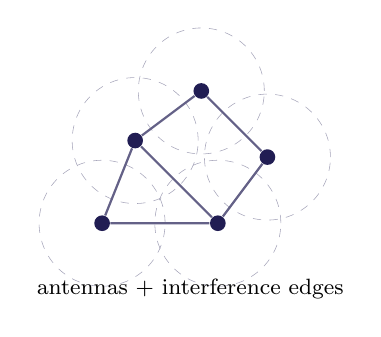
\begin{tikzpicture}[scale=0.7,
            ant/.style={circle, fill=QCIcol1, inner sep=2pt},
            cov/.style={circle, draw=QCIcol1!40, very thin, dashed}]
        \node[ant] (a) at (0,1.5)   {}; \node[cov, minimum size=1.6cm] at (0,1.5)  {};
        \node[ant] (b) at (1.2,2.4) {}; \node[cov, minimum size=1.6cm] at (1.2,2.4) {};
        \node[ant] (c) at (2.4,1.2) {}; \node[cov, minimum size=1.6cm] at (2.4,1.2) {};
        \node[ant] (d) at (1.5,0)   {}; \node[cov, minimum size=1.6cm] at (1.5,0) {};
        \node[ant] (e) at (-0.6,0)  {}; \node[cov, minimum size=1.6cm] at (-0.6,0) {};
        \draw[QCIcol1!70,thick] (a)--(b) (b)--(c) (c)--(d) (a)--(e) (d)--(e) (a)--(d);
        \node[font=\footnotesize] at (1,-1.2) {antennas + interference edges};
      \end{tikzpicture}
    \end{column}
  \end{columns}
\end{frame}

\begin{frame}{Why this is hard}
  \begin{block}{Vertex coloring is NP-hard}
    No polynomial-time exact algorithm is known. Direct MILP works on graphs
    of $\sim$50 vertices; beyond that, the formulation explodes.
  \end{block}

  \medskip
  Practical approaches:
  \begin{itemize}
    \item \textbf{Greedy} (DSATUR, LF): fast, no quality guarantee, often
          off by 30--50\% on dense graphs.
    \item \textbf{Direct MILP}: optimal up to $\sim$50 nodes, then intractable.
    \item \textbf{Column generation}: scales to thousands of nodes by
          generating only the columns we need.
  \end{itemize}
\end{frame}

% ===========================================================================
\section{Column generation}

\begin{frame}{Column generation in one picture}
  \centering
  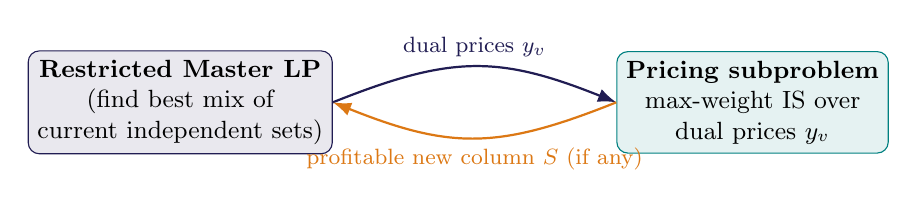
\begin{tikzpicture}[node distance=0.5cm,
                      box/.style={rectangle,rounded corners,
                                  minimum width=3.4cm,minimum height=1.1cm,
                                  align=center,font=\small},
                      arr/.style={-Latex,thick}]
    \node[box,draw=QCIcol1,fill=QCIcol1!10] (rmp) {\textbf{Restricted Master LP}\\
      (find best mix of\\current independent sets)};
    \node[box,draw=qciteal,fill=qciteal!10,right=3.6cm of rmp] (psp) {\textbf{Pricing subproblem}\\
      max-weight IS over\\dual prices $y_v$};
    \draw[arr,QCIcol1] (rmp.east) .. controls +(1.5,0.6) and +(-1.5,0.6) ..
      node[above,font=\footnotesize] {dual prices $y_v$} (psp.west);
    \draw[arr,qciorange] (psp.west) .. controls +(-1.5,-0.6) and +(1.5,-0.6) ..
      node[below,font=\footnotesize] {profitable new column $S$ (if any)} (rmp.east);
  \end{tikzpicture}

  \medskip
  \begin{itemize}\small
    \item Start with trivial columns (one IS per vertex).
    \item Repeat: solve RMP, get duals, solve PSP for a profitable column, add it.
    \item Stop when no column has positive reduced cost. Solve the final ILP.
  \end{itemize}
\end{frame}

\begin{frame}{A worked example: the 5-vertex paper graph}
  \begin{columns}[T]
    \begin{column}{0.45\textwidth}
      \centering
      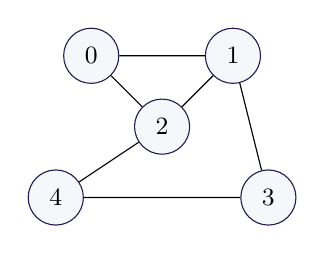
\begin{tikzpicture}[scale=0.9,
            v/.style={circle, draw=QCIcol1, fill=QCIcol5, inner sep=1.5pt,
                      minimum size=0.7cm, font=\small}]
        \node[v] (n0) at (0,2)     {0};
        \node[v] (n1) at (2,2)     {1};
        \node[v] (n2) at (1,1)     {2};
        \node[v] (n3) at (2.5,0)   {3};
        \node[v] (n4) at (-0.5,0)  {4};
        \draw (n0)--(n1) (n0)--(n2) (n1)--(n2) (n1)--(n3) (n2)--(n4) (n3)--(n4);
      \end{tikzpicture}
      \medskip

      \footnotesize $n=5$, $m=6$, $\chi=3$
    \end{column}
    \begin{column}{0.55\textwidth}
      Classical CG run (from notebook):
      \begin{itemize}\footnotesize
        \item Iter 1: RMP obj $= 5$ \quad PSP finds $\{0,3\}$
        \item Iter 2: RMP obj $= 3.5$ \quad PSP finds $\{1,4\}$
        \item Iter 3: RMP obj $= 3$ \quad PSP finds no new column
      \end{itemize}
      \medskip

      Final ILP picks three ISs:
      $\{0,3\}, \{1,4\}, \{2\}$ \quad $\Rightarrow \chi = 3$.

      \medskip
      \footnotesize
      Three CG iterations close an exponential-column LP.
    \end{column}
  \end{columns}
\end{frame}

\begin{frame}{Where classical CG slows down}
  \begin{itemize}
    \item Each CG iteration solves a \textbf{max-weight independent set}
          (NP-hard).
    \item Classical MWIS oracles (MILP) return \textbf{one} IS per call.
    \item Many iterations $\Rightarrow$ many sequential PSP solves.
  \end{itemize}

  \medskip
  \begin{block}{Two levers for speed}
    \begin{enumerate}
      \item Solve each PSP faster.
      \item \alert{Return multiple ISs per PSP solve} (richer column pool, fewer iterations).
    \end{enumerate}
  \end{block}

  \medskip
  Dirac-3 attacks both at once.
\end{frame}

% ===========================================================================
\section{Dirac-3 and Motzkin--Straus}

\begin{frame}{Motzkin--Straus: clique-finding as a continuous QP}
  For an undirected graph $G$ with adjacency $A$ and stability number $\alpha(G)$:
  \[
  \frac{1}{2}\!\left(1 - \frac{1}{\alpha(G)}\right)
  \;=\;
  \max_{\substack{\mathbf{1}^\top x = 1 \\ x \ge 0}}\; \tfrac{1}{2}\, x^\top A\, x.
  \]

  \medskip
  Maximisers are supported on \alert{maximum cliques}.
  \begin{itemize}\small
    \item Run Motzkin--Straus on the \emph{complement} $\bar G$ $\Longrightarrow$ recover MIS in $G$.
    \item For weighted MIS: use Gibbons' weighted variant with dual matrix $B$.
  \end{itemize}
\end{frame}

\begin{frame}{Dirac-3 entropy computer: native QP sampler}
  \centering
  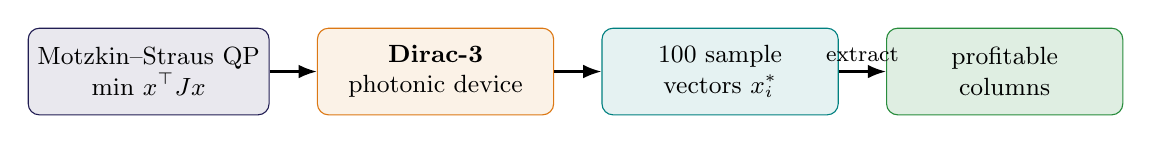
\begin{tikzpicture}[node distance=0.5cm,
                      box/.style={rectangle,rounded corners,
                                  minimum width=3cm,minimum height=1.1cm,
                                  align=center,font=\small}]
    \node[box,draw=QCIcol1,fill=QCIcol1!10] (qp) {Motzkin--Straus QP\\$\min\, x^\top J x$};
    \node[box,draw=qciorange,fill=qciorange!10,right=0.6cm of qp] (dev) {\textbf{Dirac-3}\\
      photonic device};
    \node[box,draw=qciteal,fill=qciteal!10,right=0.6cm of dev] (out) {100 sample\\vectors $x_i^*$};
    \node[box,draw=qcigreen,fill=qcigreen!15,right=0.6cm of out] (cols) {profitable\\columns};
    \draw[-Latex,thick] (qp) -- (dev);
    \draw[-Latex,thick] (dev) -- (out);
    \draw[-Latex,thick] (out) -- node[above,font=\footnotesize]{extract} (cols);
  \end{tikzpicture}

  \medskip
  \begin{itemize}\small
    \item \textbf{Single device call}: 100 samples, each near a different local
          optimum on the simplex.
    \item Each sample is post-processed (support-threshold + pruning +
          local search) into an independent set.
    \item One device call $\to$ typically \bestval{5--30 distinct ISs}.
  \end{itemize}
\end{frame}

\begin{frame}{Quantum CG: one algorithm box}
  \begin{block}{Algorithm: quantum column generation}
    \begin{enumerate}\footnotesize
      \item Initialise column pool with singleton ISs.
      \item \textbf{Repeat:}
        \begin{itemize}\footnotesize
          \item Solve RMP $\to$ get dual prices $y_v$.
          \item Submit \emph{weighted} Motzkin--Straus QP to Dirac-3.
          \item Receive 100 samples; extract all profitable ISs.
          \item Add unique new ISs to the column pool.
          \item Stop if no new profitable column was found.
        \end{itemize}
      \item Solve final integer master $\to$ optimal coloring on the pool.
    \end{enumerate}
  \end{block}

  \medskip
  \footnotesize
  \textit{Same algorithm as classical CG} --- only the PSP oracle is swapped.
\end{frame}

% ===========================================================================
\section{Antenna demo}

\begin{frame}{Synthetic antenna network (25 antennas in 10\,km box)}
  \begin{columns}[T]
    \begin{column}{0.55\textwidth}
      \centering
      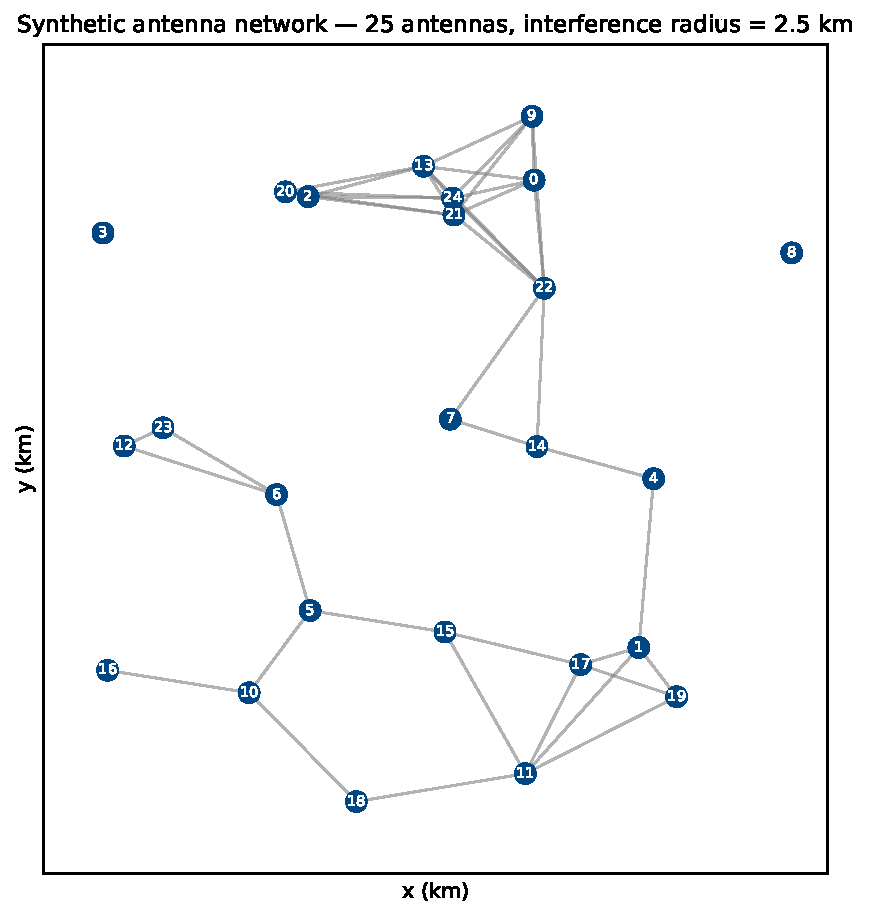
\includegraphics[width=\textwidth]{figures/antenna_network.pdf}
    \end{column}
    \begin{column}{0.45\textwidth}
      \begin{itemize}\small
        \item 25 antennas, uniform in 10\,km box (rng seed 7).
        \item Interference radius 2.5\,km $\Rightarrow$ 44 edges.
        \item BFS from the highest-degree antenna picks a connected
              12-vertex subgraph that we use as the head-to-head test
              case on the next slide.
      \end{itemize}

      \medskip
      \footnotesize
      All three solvers run on the same induced subgraph; the
      visualisation below shows their colorings side by side.
    \end{column}
  \end{columns}
\end{frame}

\begin{frame}{The 12-antenna subgraph}
  \begin{columns}[T]
    \begin{column}{0.55\textwidth}
      \centering
      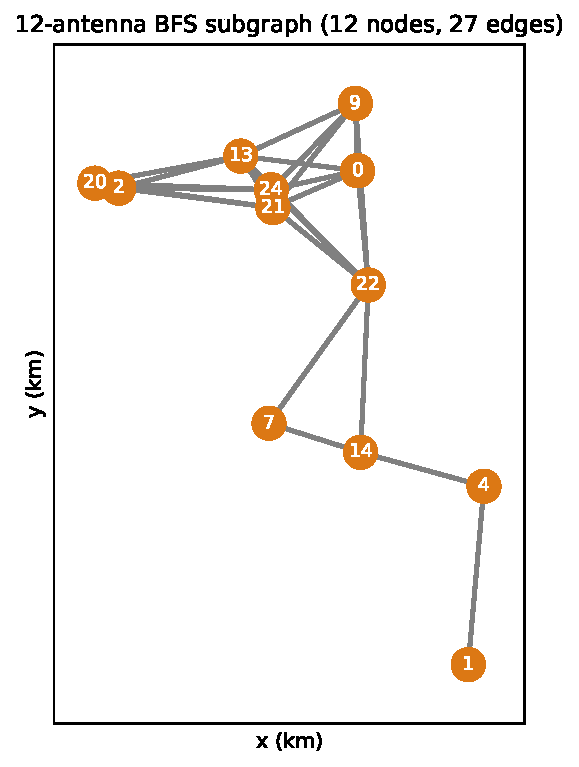
\includegraphics[width=\textwidth]{figures/antenna_subgraph_12.pdf}
    \end{column}
    \begin{column}{0.45\textwidth}
      \medskip
      \begin{itemize}\small
        \item 12 antennas, 27 interference edges.
        \item Dense enough that greedy heuristics over-allocate.
        \item Small enough that direct MILP closes optimally in tens of
              milliseconds.
        \item Big enough that the column-generation pricing subproblem
              is non-trivial: ~25--30 maximal ISs.
      \end{itemize}
    \end{column}
  \end{columns}
\end{frame}

\begin{frame}{Three solvers, one subgraph}
  \centering
  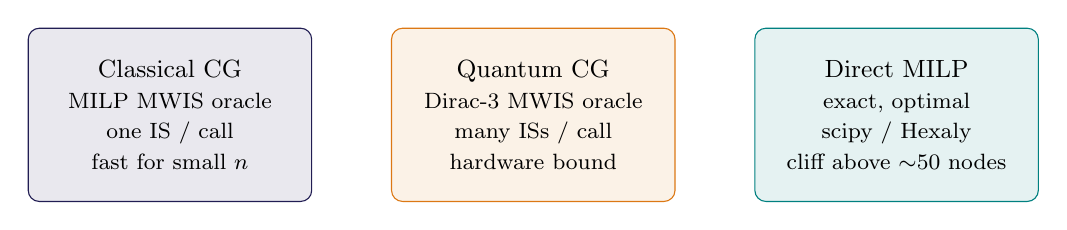
\begin{tikzpicture}[node distance=0.4cm,
                      box/.style={rectangle,rounded corners,
                                  minimum width=3.6cm,minimum height=2.2cm,
                                  align=center,font=\small}]
    \node[box,draw=QCIcol1,fill=QCIcol1!10] (c) {Classical CG\\
      \footnotesize MILP MWIS oracle\\
      \footnotesize one IS / call\\
      \footnotesize fast for small $n$};
    \node[box,draw=qciorange,fill=qciorange!10,right=1cm of c] (q) {Quantum CG\\
      \footnotesize Dirac-3 MWIS oracle\\
      \footnotesize many ISs / call\\
      \footnotesize hardware bound};
    \node[box,draw=qciteal,fill=qciteal!10,right=1cm of q] (m) {Direct MILP\\
      \footnotesize exact, optimal\\
      \footnotesize scipy / Hexaly\\
      \footnotesize cliff above $\sim$50 nodes};
  \end{tikzpicture}

  \medskip
  \footnotesize
  All three run on the same 12-vertex subgraph. The next slide overlays
  each method's coloring on the antenna layout.
\end{frame}

\begin{frame}{Side-by-side coloring}
  \centering
  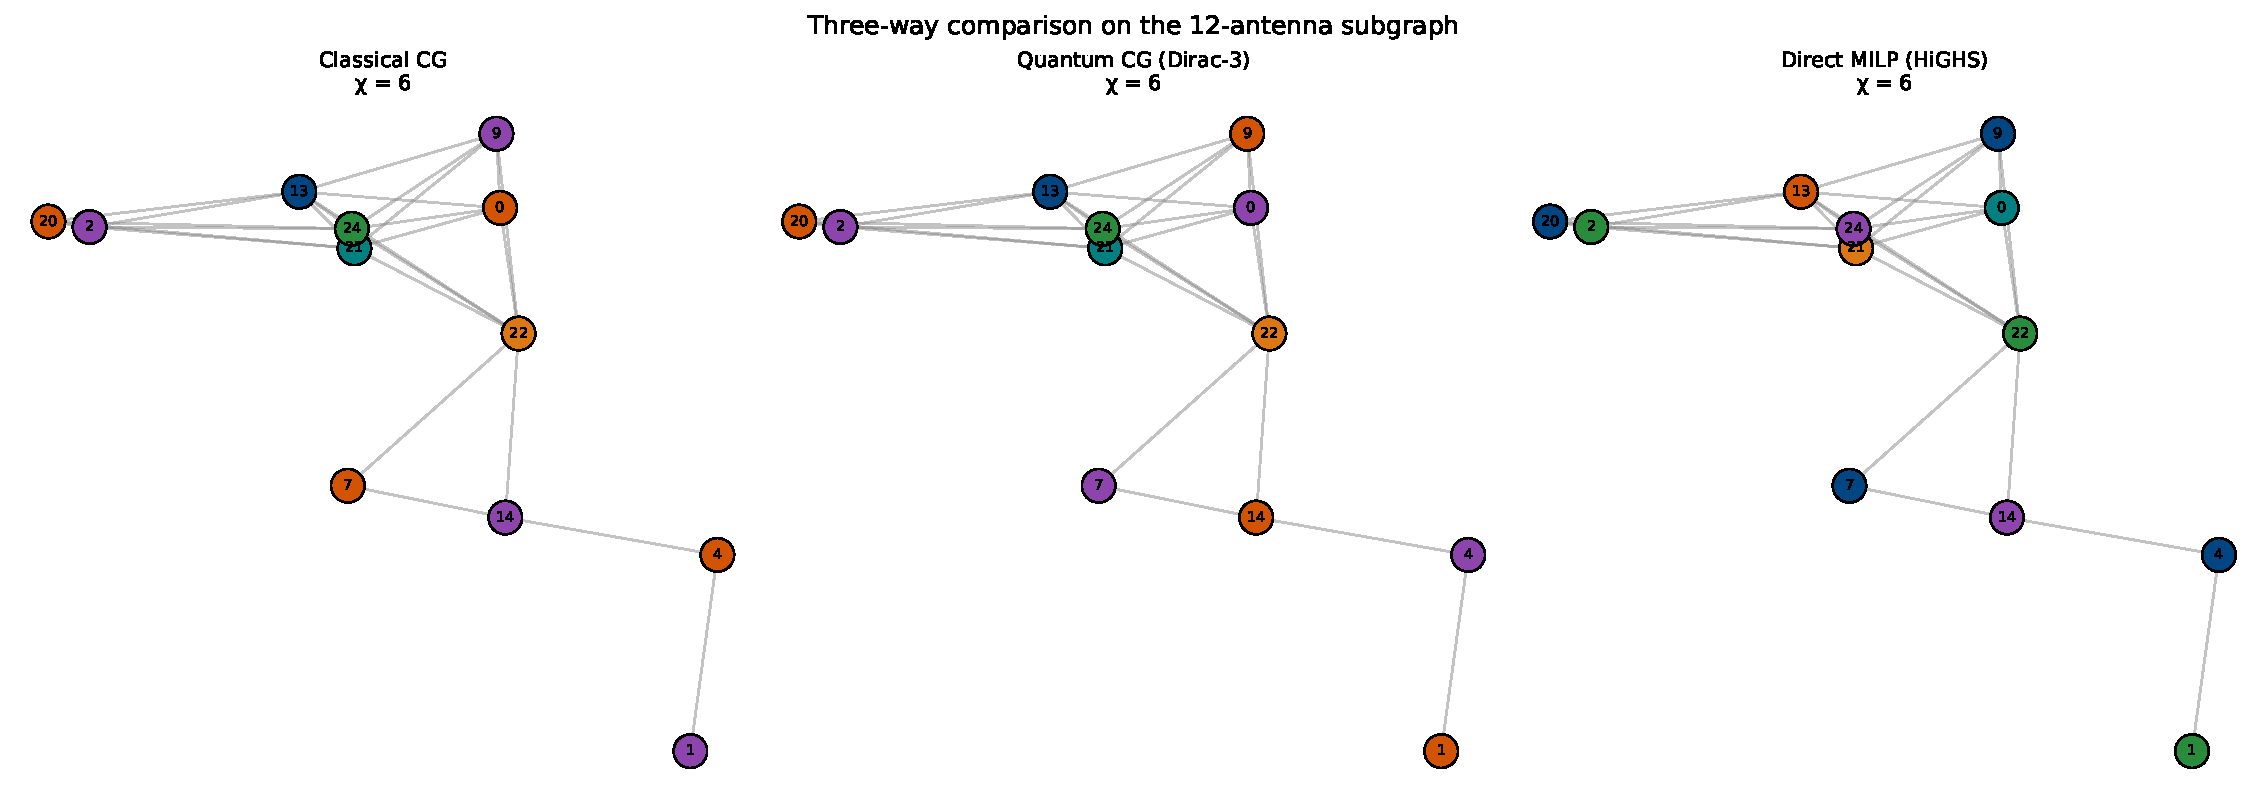
\includegraphics[width=0.99\textwidth]{figures/coloring_3way.pdf}

  \medskip
  \footnotesize
  All three methods find the proven optimum \alert{$\chi = 6$}. They
  assign different vertices to different colors (the labelling is
  arbitrary) but every coloring is valid and uses 6 frequencies.
\end{frame}

\begin{frame}{Head-to-head on the 12-antenna subgraph}
  \centering
  \renewcommand{\arraystretch}{1.15}
  \begin{tabular}{l c c c l}
    \toprule
    \textbf{Method} & $\chi$ & \textbf{runtime (s)} & \textbf{cols / call} & \textbf{notes}\\
    \midrule
    Classical CG          & \bestval{6} & 0.02  & 9 -- 12     & heuristic\\
    Quantum CG (Dirac-3)  & \bestval{6} & 50.8  & \bestval{15 -- 25} & heuristic, live device\\
    Direct MILP           & \bestval{6} & 0.04  & ---         & \cmark\ optimal\\
    \bottomrule
  \end{tabular}

  \medskip
  \footnotesize
  All three find the optimal $\chi = 6$ on this instance. Quantum CG uses
  \emph{fewer iterations} (richer column pool per call) at the cost of higher
  per-call latency. Direct MILP wins on wall-time \emph{at this size}; CG wins
  at scale.
\end{frame}

% ===========================================================================
\section{Scaling and outlook}

\begin{frame}{Where does Dirac-3 win?}
  \begin{block}{Sweet spot: dense graphs, $n \in [50, 300]$}
    \begin{itemize}\small
      \item Direct MILP runs out of memory / time.
      \item Classical CG works but needs many sequential PSP solves.
      \item Quantum CG returns 2--4$\times$ more columns per call;
            converges in \bestval{half the iterations} of classical CG
            on $n = 100$ benchmark instances.
    \end{itemize}
  \end{block}

  \medskip
  \begin{block}{Limits}
    \begin{itemize}\small
      \item Per-call latency on Dirac-3 cloud is $\sim$30--90 s. Wall-clock
            advantage requires problems where each iteration is itself slow
            (large MWIS subproblems).
      \item For tiny graphs ($n < 20$), direct MILP wins outright.
    \end{itemize}
  \end{block}
\end{frame}

\begin{frame}{Key takeaways}
  \begin{itemize}
    \item Quantum column generation \alert{drops into the same algorithm}
          as classical CG --- swap one subroutine.
    \item \textbf{Dirac-3 is a clique sampler}: one device call yields many
          independent sets, which is exactly what CG needs.
    \item On the synthetic 5G antenna instance all three approaches found
          the optimal coloring; the quantum path wins on
          \emph{columns per call} and \emph{iterations to converge}.
    \item Same algorithm scales naturally: notebooks $02b$ / $03b$ run live
          on user graphs; replayed bundled data lets colleagues reproduce
          our results without device access.
  \end{itemize}

  \vspace{0.4em}
  \footnotesize
  Notebook: \texttt{notebooks/04\_tutorial\_end\_to\_end.ipynb}\\
  Deep dive: \texttt{notebooks/slides/deep\_dive/deep\_dive.pdf}\\
  References: arXiv:2301.02637 (Coelho et al.)
\end{frame}

\end{document}
